\documentclass[a4paper,12pt]{article}

\usepackage[english]{babel}
\usepackage[T1]{fontenc}
\usepackage[utf8]{inputenc}
\usepackage{amsmath}
\usepackage{amsthm}
\usepackage{forest}
\usepackage{graphicx}
\graphicspath{{images/}}
\usepackage{tikz}
\usepackage{tikz-qtree}
\usepackage{graphicx}
\usepackage{xcolor}
\usepackage[colorinlistoftodos]{todonotes}
\usepackage{enumitem}
\usepackage{DejaVuSansMono}
\usepackage{listings}
\lstset{basicstyle=\footnotesize\ttfamily,breaklines=true}
\lstset{frame=tb,language=python,numbers=left,showstringspaces=false}
\renewcommand{\lstlistingname}{Code Block}

\usepackage{geometry}
\geometry{total={210mm,297mm},
left=20mm, right=20mm,
bindingoffset=0mm,
top=20mm, bottom=20mm}

\usepackage[
  pdftitle={Assignment 4},
  pdfauthor={William Jagels},
  colorlinks=true,linkcolor=blue,urlcolor=blue,citecolor=blue,bookmarks=true,
bookmarksopenlevel=2]{hyperref}

\usepackage{titlesec}
\titlelabel{\thetitle.\quad}

\def\code#1{\texttt{#1}}

\title{Assignment 4}

\author{William Jagels}

\date{\today}

\begin{document}
\maketitle

\section{}
Pseudocode:
\begin{lstlisting}
def asquared(A):
  for i, j in A:
    n = 1
    while A[i, j] != 1 and n < len(A):
      if A[i, n] and A[n, j]:
        A[i, j] = 1
      n += 1
  return A
\end{lstlisting}
$\Theta(N^3)$
\section{}
\begin{enumerate}
  \item To find a cycle, perform DFS and check whether or not the node was visited, and if
    the node was visited but not where we were last (parent node), then there is a cycle.
    This can be done with a standard adjacency matrix.
  \item Again, you can use DFS and use an array to mark each node as visited.
    At the end of the DFS, check that the array indicates that every node was visited.
    If any nodes were not visited during the DFS, then we know that the graph is disconnected.
    To determine whether or not the graph is a tree, simply apply the cycle checking and
    connectivity, if both are true, then the graph is a tree.
    In the below example, we'll notice that $\{D, H, G\}$ will not be visited if we start at
    node $A$, therefore it's not a tree.
\end{enumerate}
\section{Does an undirected graph with 5 vertices, each of degree 3 exist?}
No, because the sum of degrees in a graph must be even.
With $|V| = 5$ and the sum of degrees being equal to $2|E|$, the number of edges would have
to be $\frac{15}{2}$.
The number of edges has to be an integer, so this situation can never happen.
\section{}
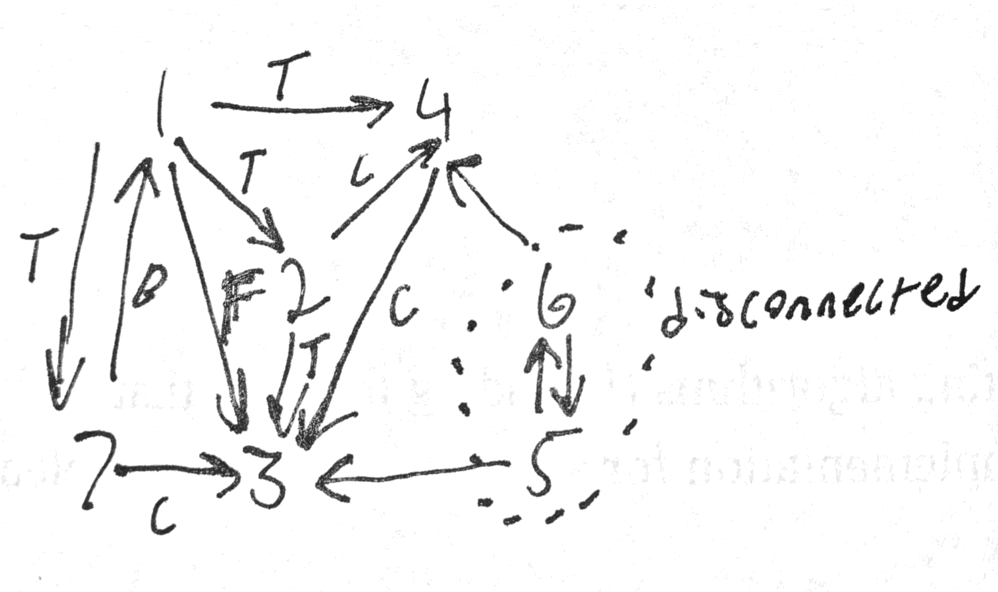
\includegraphics[width=10cm]{bfs}
\section{}
Sorted: 1 7 2 4 3 8

1: discovered: 1, finished: 3

7: discovered: 2, finished: 5

2: discovered: 3, finished: 5

4: discovered: 4, finished: 6

3: discovered: 5, finished: 5

8: discovered: 6, finished: 6

\section{}
To check for a bipartition, check if the graph is 2-colorable.

Pseudocode:
\begin{lstlisting}
def isbipartite(node):
  if not node.color:
    node.color = RED
  for nbr in node.neighbors:
    if nbr.color == node.color:
      return false
    nbr.color = opposite(node.color)
    if not isbipartite(nbr):
      return false
  return true
\end{lstlisting}
The disjoint sets $V_1, V_2$ can be seen by extracting red and blue vertices.
This particular graph is bipartite.

$V_0 = \{1, 4, 5, 6, 7, 11\}$

$V_1 = \{2, 3, 8, 9, 10\}$

\section{}
\begin{enumerate}
  \item a bfs: $1, 2, 4, 7, 3, 5, 6$

    b bfs: $1, 2, 4, 5, 3, 6, 7$
  \item a dfs: $1, 2, 7, 3, 4, 5, 6$

    b dfs: $1, 2, 3, 4, 6, 5, 7$
\end{enumerate}

\section{}
\begin{enumerate}
  \item 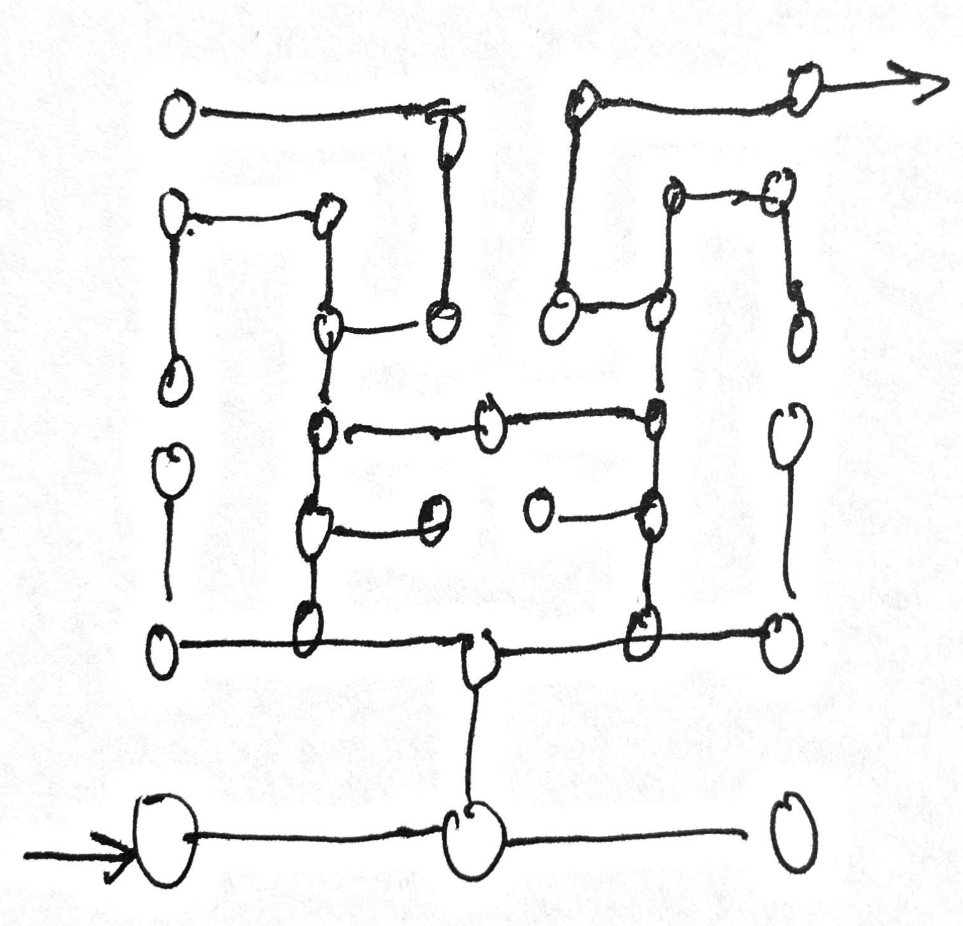
\includegraphics[width=15cm]{maze}
  \item DFS because you want to get out of the maze quickly, and finding the optimal
    isn't needed.
\end{enumerate}
\section{}
\begin{enumerate}
  \item $z = 3x + 2y$ is maximized when $x=3$, $y=4$
    The minimum occurs at $x=0$, $y=0$.
  \item $z = 4x + 3y$ is maximized when $x=5$, $y=3$
    The minimum occurs at $x=0$, $y=2$.
\end{enumerate}
\section{}
Setup equations
$$
  45a + 50b = Profit,\\
  250a + 400b \leq 70000,\\
  a + b \leq 250
$$
Maximizing profit, we get $a = 200, b = 50$.
Which means the merchant should produce $200$ low cost computers and $50$ high cost ones.


\end{document}
